\documentclass{article}

% Document extensibility %
%
% Disables native paragraph indentation
\usepackage{parskip} 
%
% Provides further bullet options for lists
\usepackage{enumitem}

% Mathematical symbol and statement packages %
%
% Necessary
\usepackage{amsmath}
\usepackage{amssymb}
%
% Extensive fraction notation
\usepackage{xfrac}
%
% Generic mathematical commands
% Notable: \degree, \celcius
\usepackage{gensymb}
%
% Variable vector notation (arrow above variable)
\usepackage{esvect}
%
% Multiline boxed equations
\usepackage{empheq}
%
% SI Unit
\usepackage{siunitx}
%
% More intuitive arrays/matrices
\usepackage{array}

% Graphic packages %
%
% Diagrams and illustrations
\usepackage{tikz}
\usetikzlibrary{positioning}
%
% Image insertion
\usepackage{graphicx}

% Document content %
%
% Change title of table of contents
% \renewcommand{\contentsname}{Title}

\begin{document}

% Command `\hr` to insert horizontal rules
\newcommand{\hr}{\par\noindent\rule{\textwidth}{0.4pt}}

% Command to box and center math equations
\newcommand{\bc}[1]{
	\begin{equation*}
		\begin{boxed}
			{#1}
		\end{boxed}
	\end{equation*}
}

% Command for single line equations with a condition
\newcommand{\cond}[2]{
	\ifmmode
		{#1} \quad {#2}
	\else
		$$ {#1} \quad {#2} $$
	\fi
}

\tableofcontents

\section{Energy}

\subsection{Review: Dot Product}
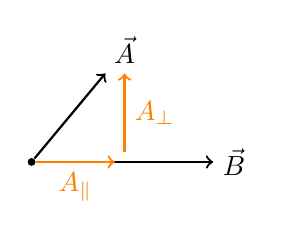
\begin{tikzpicture}
	\node[circle, fill, inner sep = 1pt] (origin) {};
	\node (result) [right = of origin] {};
	\node (A) [above = of result] {$ \vec{A} $};
	\node (B) [right = of result] {$ \vec{B} $};

	\draw[black, thick, ->] (origin) -- (B);
	\draw[orange, thick, ->] (origin) -- (result) node [midway, below] {$ A_{\parallel} $};
	\draw[black, thick, ->] (origin) -- (A);
	\draw[orange, thick, ->] (result) -- (A) node [midway, right] {$ A_\perp $};
\end{tikzpicture}

$$ \vec{A} \cdot \vec{B} = AB $$
if $ \vec{A} $ \& $ \vec{B} $ are already $ \parallel $
$$ \vec{A} \cdot \vec{B} = AB $$

if $ A $ \& $ B $ are $ \perp $ then $ \vec{A} \cdot \vec{B} = 0 $.

\hr

Dot Product: How much of $ \vec{A} $ is applied to $ \vec{B} $?

Work
\begin{itemize}
	\item by definition, is the \underline{work} done by a force over a path.
	\item is a measure of how much a force acts on a mass for the duration of a displacement.
	\item 's unit is:
		\begin{enumerate}
			\item MKS - J (Joule)
			\item CGS - erg
		\end{enumerate}
\end{itemize}
An amount of work is called ``Energy"

$$ W = \int \vec{F} \cdot d\vec{x} $$
\begin{enumerate}
	\item $ W $ is ``work"
	\item $ \vec{F} $ is the \textbf{applied force}
	\item $ d\vec{x} $ is the \textbf{displacement along a path}
\end{enumerate}

\subsection{Line Element}

Consider force:
$$ \vec{F} = (\SI{2}{\newton \per \meter})x \hat{x} + (\SI{1}{\newton \per \meter \squared})xy \hat{y} $$

Recall: $$ \vec{A} \cdot \vec{B} = A_xB_x + A_yB_y $$
$ d\vec{x} $ is called the ``line element" and is tied to the coordinate system.

The line element \textbf{never} changes!
$$ d\vec{x} = dx \hat{x} + dy \hat{y} + dz \hat{z} $$
\begin{equation}
	d\hat{x} = dr \hat{r} + rd\theta \hat{\theta} + dz \hat{z}
\end{equation}
\begin{align*}
	\hat{F} \cdot d\hat{x} & = F_xdx + F_ydy + F_zdz \\
						   & = (\SI{2}{\newton \per \meter})xdx + (\SI{1}{\newton \per \meter \squared})xydy
\end{align*}
Always substitute so you are integrating one variable.

The path of integration \textit{is} the substitution.
\begin{align*}
	y & = 3x + 2m \\
	dy & = 3dx
\end{align*}
Now we can solve the integral
\begin{align*}
	W & = \int_C \vec{F} \cdot d\vec{x} \\
	  & = \int_C (\SI{2}{\newton \per \meter})dx + \int_C (\SI{1}{\newton \per \meter \squared})xydy \quad \text{(Substitute)} \\
	  & = \int_0^{3m} (\SI{2}{\newton \per \meter})xdx + \int_0^{3m} (\SI{1}{\newton \per \meter \squared})(x)(3x + 2m)(3)dx \\
	W & = \frac{\SI{2}{\newton \per \meter}}{2}x^2 \biggr\rvert_0^{3m} + \SI{3}{\newton \per \meter \squared} \int_0^{3m} 3x^2 dx + \SI{3}{\newton \per \meter \squared} \int_0^{3m} (\SI{2}{\meter})xdx \\
	  & = \SI{9}{\newton \meter} + (\SI{3}{\newton \per \meter})x^3 \biggr\rvert_0^{3m} + (\SI{3}{\newton \per \meter})x^2 \biggr\rvert_0^{3m} \\
	  & = \SI{9}{\newton \meter} + \SI{81}{\newton \meter} + \SI{27}{\newton \meter} \\
	W & = \SI{117}{\newton \meter}
\end{align*}
\bc{W = \SI{117}{\joule}}

\subsection{Forces \& Work}

For forces that are uniform
$$ \text{uniform: } \frac{df}{dx} = 0 $$
$$ \text{constant: } \frac{df}{dt} = 0 $$
\begin{align*}
	W & = \int \vec{F} \cdot d\vec{x} \\
	W & = \vec{F} \cdot \int d\vec{x} \\
	W & = \vec{F} \cdot \Delta \vec{x}
\end{align*}

\hr

\textbf{Example of Finding Work}

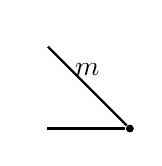
\begin{tikzpicture}
	\node[fill, circle, inner sep = 1pt] (origin) {};
	\node (slant) [above left = of origin] {};
	\node (floor) [left = of origin] {};

	\draw[black, thick] (origin) -- (slant) node [midway, above] {$ m $};
	\draw[black, thick] (origin) -- (floor);
\end{tikzpicture}
\begin{align*}
	m & = \SI{1}{\kilogram} \\
	\theta & = \SI{40}{\degree} \\
	\mu_k & = 0.7 \\
	\Delta x & = \SI{19}{\meter} \\
	mg & = \SI{10}{\newton}
\end{align*}
\begin{align*}
	\sum F_y & = 0 \\
	N - mg\cos(\theta) & = 0 \\
	N & = mg\cos(\theta) \\
	  & = (\SI{10}{\newton})\cos(\SI{40}{\degree}) \\
	N & = \SI{7.7}{\newton}
\end{align*}
\begin{align*}
	f & = \mu N \\
	  & = (0.7)(\SI{7.7}{\newton}) \\
	f & = \SI{5.4}{\newton}
\end{align*}
Calculate the work for each force:
\begin{align*}
	W_N & = \vec{F}_N \cdot \Delta \vec{x} \\
		& = (0 \hat{x} + \SI{7.7}{\newton} \hat{y}) \cdot (\SI{19}{\meter} \hat{x} + 0 \hat{y}) \\
	W_N & = 0
\end{align*}
\begin{align*}
	W_{mg} & = m\vec{g} \cdot \Delta \hat{x} \\
		   & = \left[ mg\sin(\theta) \hat{x} + (-mg\cos(\theta)) \hat{y} \right] \cdot \left[ \Delta x \hat{x} + 0 \hat{y} \right] \\
	W_{mg} & = mg\Delta x\sin(\theta) \\
		   & = (\SI{10}{\newton})(\SI{19}{\meter})\sin(\SI{40}{\degree}) \\
	W_{mg} & = \SI{122}{\joule}
\end{align*}
\begin{align*}
	W_f & = \vec{f} \cdot \Delta \vec{x} \\
		& = (-\SI{5.4}{\newton} \hat{x}) \cdot (\SI{19}{\meter} \hat{x}) \\
	W_f & = -\SI{103}{\joule}
\end{align*}
\bc{W_N = 0, W_{mg} = \SI{122}{\joule}, W_f = -\SI{103}{\joule}}
\begin{itemize}
	\item $ W > 0 \rightarrow $ Speeds system up
	\item $ W < 0 \rightarrow $ Slows system up
	\item $ W = 0 \rightarrow \Delta v = 0 $
	\item Net work $ \sum W_i $ is indicative of the overall motion
\end{itemize}
\begin{align*}
	W_\text{net} & = \sum W_i \\
				 & = W_{mg} + W_N + W_f \\
				 & = \SI{122}{\joule} + 0 - \SI{103}{\joule} \\
	W_\text{net} & = \SI{19}{\joule}
\end{align*}
\bc{W_\text{net} = \SI{19}{\joule}}

\hr

How is work related to speed?
\begin{align*}
	W & = \int \vec{F} \cdot d\vec{x}
\end{align*}
Consider 1D case where $ \cos(\theta) \rightarrow 1 $
\begin{align*}
	W & = \int \left( F \right) dx \\
	  & = \int \left( ma \right) dx \\
	  & = \int \left( m\frac{dv}{dt} \right) dx \\
	  & = \int \left( mdv \left( \frac{dx}{dt} \right) \right) \\
	  & = \int \left( mv \right) dv \\
	  & = \int_{v_i}^{v_f} \left( mv \right) dv \\
	  & = \frac{1}{2}mv^2 \biggr\rvert_{v_i}^{v_f} \\
	W & = \frac{1}{2}mv_f^2 - \frac{1}{2}mv_i^2
\end{align*}

Energy is associated with speed is called \textbf{Kinetic Energy (KE)}
$$ \text{KE} = \frac{1}{2}mv^2 $$
is the kinetic energy of translation.

Work is also defined as $$ W = \Delta \text{KE} $$
this is called the \textbf{Work-Kinetic Energy Theorem}

if the block started from rest:
\begin{align*}
	W & = \frac{1}{2}mv_f^2 - 0 \\
	v_f & = \sqrt{\frac{2W_\text{net}}{m}} \\
		& = \sqrt{\frac{2(\SI{19}{\joule})}{\SI{1}{\kilogram}}} \\
	v_f & = \SI{6.2}{\meter \per \second}
\end{align*}
\bc{v_f = \SI{6.2}{\meter \per \second}}
(Using the graph from above)
\begin{align*}
	\sin(\theta) & = \frac{h}{\Delta x} \\
	h & = \Delta x\sin(\theta) \\
	h & = (\SI{19}{\meter})\sin(\SI{40}{\degree}) \\
	h & = \SI{12.2}{\meter}
\end{align*}
How does the answer change if there is no friction?
\begin{align*}
	W_\text{net} & = W_{mg} + W_N \\
				 & = \SI{122}{\joule} + 0 \\
	W_\text{net} & = \SI{122}{\joule}
\end{align*}

\hr

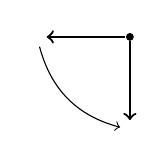
\begin{tikzpicture}
	\node[fill, circle, inner sep = 1pt] (origin) {};
	\node (x) [left = of origin] {};
	\node (y) [below = of origin] {};

	\draw[black, thick, ->] (origin) -- (x);
	\draw[black, thick, ->] (origin) -- (y);
	\draw[bend right, ->] (x) to (y);
\end{tikzpicture}

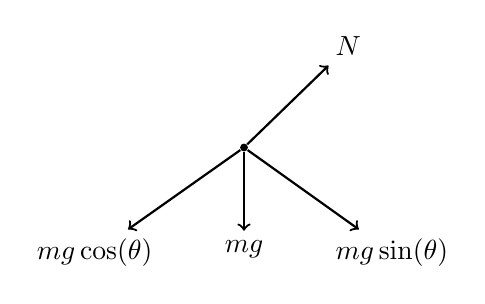
\begin{tikzpicture}
	\node[fill, circle, inner sep = 1pt] (origin) {};
	\node (below_left) [below left = of origin] {$ mg\cos(\theta) $};
	\node (below) [below = of origin] {$ mg $};
	\node (below_right) [below right = of origin] {$ mg\sin(\theta) $};
	\node (above_right) [above right = of origin] {$ N $};

	\foreach \node in {below_left, below, below_right, above_right}
		\draw[black, thick, ->] (origin) -- (\node);
\end{tikzpicture}
\begin{align*}
	W_N & = 0
\end{align*}
\begin{align*}
	W_{mg} & = \int \left( mg\cos(\theta) \hat{r} + mg\sin(\theta) \hat{\theta} \right) \cdot \left( dr \hat{r} + rd\theta \hat{\theta} \right) \\
		   & = \int \left( mg\cos(\theta) \hat{r} + mg\sin(\theta) \hat{\theta} \right) \cdot \left( (0) \hat{r} + rd\theta \hat{\theta} \right) \\
		   & = \int_0^{\SI{90}{\degree}} mgr\sin(\theta) d\theta \\
	W_{mg} & = mgr\cos(\theta) \biggr\rvert_0^{\SI{90}{\degree}} \\
		   & = mgr\cos(\theta) \biggr\rvert_{\SI{90}{\degree}}^0 \\
	W_{mg} & = mgr \\
		   & = (\SI{10}{\newton})(\SI{12.2}{\meter}) \\
	W_{mg} & = \SI{122}{\joule}
\end{align*}
For the case of gravity, it would seem that only $ mg $ and the change in height dictate work.
\begin{align*}
	W & = \int \vec{F} \cdot d\hat{x} \\
	  & = \int mg \hat{y} \cdot (dx \hat{x} + dy \hat{y}) \\
	W & = \int_0^h mg dy \\
	W & = mgh
\end{align*}
Gravity is completely path independent.

\textbf{Conservative force} - Work is path independent

If you can write a function of position called a \textbf{Potential Energy Function} whose derivative equals force, then the force is conservative.
\begin{align*}
	\text{PE}_g & = mgy \\
	-\frac{d \left( \text{PE}_g \right)}{dy} \hat{y} & = -mg \hat{y} = \vec{F}_g \\
\end{align*}

\end{document}
